%% ------------------------------------------------------------------- %%
%% ------------------------------------------------------------------- %%
\chapter{Introducción}
\label{cap:introduccion}
\lhead{\emph{Introducción}}  % Change the left side page header to "Bibliography"


%% ------------------------------------------------------------------- %%
\section{Contexto y Motivación}
\label{sec:motivacion}

El cáncer representa el desafío de salud global más significativo \citep{siegel2023cancer}. Además, según el Instituto de Investigación del Cáncer del Reino Unido, se registraron más de 18 millones de nuevos casos y 10 millones de muertes en 2020 \citep{cancerUK2023}. Además, se predice que habrá alrededor de 28 millones de nuevos casos anualmente para alrededor de 2040 si la incidencia se mantiene estable y el crecimiento de la población y el envejecimiento continúan según las tendencias recientes \citep{cancerUK2023_2}. Esto representa un aumento del 54.9\% desde 2020, con un aumento esperado mayor en hombres (60.6\%) que en mujeres (48.8\%).

En este contexto, se sabe que los métodos tradicionales basados en cirugía, radioterapia y quimioterapia tienen baja eficacia y efectos secundarios adversos \citep{peng2019neoantigen}. Por lo tanto, ha surgido el desarrollo de la inmunoterapia contra el cáncer, con el objetivo de estimular el sistema inmunológico del paciente \citep{borden2022cancer}. Existen tratamientos como vacunas personalizadas, terapias con linfocitos T adoptivos e inhibidores de puntos de control inmunológico. De entre estos, las vacunas basadas en neoantígenos han mostrado un gran potencial al potenciar las respuestas de los linfocitos T y se consideran las más propensas a tener éxito \citep{borden2022cancer}. Además, los neoantígenos se utilizan en la terapia de bloqueo de puntos de control inmunológico. Los neoantígenos se consideran biomarcadores predictivos y objetivos para el tratamiento sinérgico en la inmunoterapia contra el cáncer \citep{fang2022neoantigens}.

%El cáncer representa el mayor problema de salud mundial \citep{siegel2022cancer} y es el causante líder de muertes, solo en el 2020 se registraron alrededor de 10 millones de muertes y aproximadamente cada año 400000 niños desarrollan cáncer \citep{whocancer2022}. Lamentablemente, a pesar de muchos esfuerzos por mitigar las muertes causadas por esta enfermedad, los métodos tradicionales basados en cirugías, radioterapias y quimioterapias tienen baja efectividad \citep{peng2019neoantigen}. En este contexto, surge el desarrollo de la inmunoterapia del cáncer, el cuál tiene el objetivo estimular el sistema inmune de un paciente. La idea es que nuestro propio sistema inmune sea capaz de reconocer las células de cáncer como agentes extraños y por consiguiente elimine dichas células. Existen varios enfoques y metodologías en la inmunoterapia del cáncer, de estos, la de mayor estudio y efectividad es el desarrollo de vacunas personalizadas \citep{borden2022cancer}.

%El desarrollo de vacunas personalizadas contra el cáncer es un proceso largo y depende de una correcta detección de neo antígenos. Estos neo antígenos son péptidos\footnote{Secuencias cortas de aminoacidos.} que solo se presentan en células cancerosas; entonces, el objetivo es entrenar a los linfocitos (células T) de un paciente para que estos puedan reconocer los neo antígenos y asi activar el sistema inmune.

%Determinar qué estrategia o método de detección de neo antígenos es el adecuado o en qué circunstancias conviene la aplicación de alguno, es muy importante para el desarrollo de vacunas personalizadas \citep{de2020neoantigen, peng2019neoantigen}.  Sin embargo, a pesar de los esfuerzos de los investigadores en desarrollar métodos y herramientas,  menos del 3\% de los neo antígenos detectados logran activar a las células T (sistema inmune) \citep{de2020neoantigen}. De esta forma, es relevante que se continue con la investigación y desarrollo de nuevos métodos que permitan detectar neo antígenos.

El desarrollo de vacunas personalizadas contra el cáncer es un proceso largo que depende de la detección precisa de neoantígenos (ver Figura \ref{fig:vaccines}). Estos neoantígenos son péptidos que se encuentran exclusivamente en las células cancerosas. El objetivo de un tratamiento basado en vacunas personalizadas es entrenar a los linfocitos (células T) del paciente para que reconozcan estos neoantígenos y activen el sistema inmunológico \citep{de2020neoantigen, peng2019neoantigen}. El proceso se resume en la Figura \ref{fig:vaccines_b} y consta de las siguientes fases:

\begin{enumerate}
	\item Obtener muestras de tejidos cancerosos y sanos. Ambos tejidos se secuencian para obtener ADN y/o ARN. Algunos enfoques incluyen información del \textit{immunopeptidome} obtenida mediante \textit{Mass Spectrometry} (MS).
	\item En la etapa \textit{in-silico}, se realiza el alineamiento de secuencias, se desarrolla un proceso de llamada de variantes para detectar variaciones y/o mutaciones, y se anotan estas variantes (posible detección de neoantígenos). Hay disponibles varias herramientas con buen rendimiento para esta etapa.
	\item En esta etapa \textit{in-silico}, se priorizan los neoantígenos. Este paso es crucial y ha recibido una atención significativa en la investigación en los últimos años debido a su complejidad y la baja efectividad de los enfoques actuales. Aquí, se evalúa la afinidad de los candidatos neoantígenos (péptidos) de la etapa anterior con el \textit{Major Histocompatibility Complex} (MHC), conocido como la unión pMHC. Luego, se evalúa la afinidad de pMHC para unirse al \textit{T-cell Receptor} (TCR). Al final de esta etapa, se obtienen los neoantígenos.
	\item En la etapa \textit{in-vitro}, en el laboratorio se inducen las células T del paciente para que reconozcan los neoantígenos. En este punto, se desarrollan las vacunas. Esta etapa la llevan a cabo biotecnólogos y biólogos.
	\item Finalmente, el oncólogo realiza una evaluación clínica de la vacuna.
	
\end{enumerate}

La detección \textit{in-silico} de neoantígenos se basa en las etapas segunda y tercera representadas en la Figura \ref{fig:vaccines}(b). En este contexto, debido a la complejidad del proceso y la variedad de métodos disponibles, se han desarrollado herramientas de \textit{software} y flujos de trabajo para agilizar el uso de estas herramientas. Además, los \textit{Transformers} han marcado el comienzo de una nueva era en la inteligencia artificial, demostrando logros destacados en una variedad de tareas de procesamiento del lenguaje natural  \citep{patwardhan2023transformers}. Estos modelos también han encontrado aplicación en la detección de neoantígenos, especialmente en la tercera etapa de la Figura \ref{fig:vaccines}(b). Se han propuesto modelos BERT y redes de aprendizaje profundo con mecanismos de atención para predecir la unión péptido-MHC y pMHC-TCR obteniendo resultados prometedores. Sin embargo, aún existe mucho camino por recorrer y con el incremento constante de muestras de ADN/proteínas, sumado a los nuevos mecanismos para entrenar modelos \textit{Transformers} con miles de millones de parámetros ($10^9$), se espera lograr avances significativos en este campo de estudio.


\begin{figure}[h]
	\centering
	\subfigure[Proceso de desarrollo]{\label{fig:vaccines_a}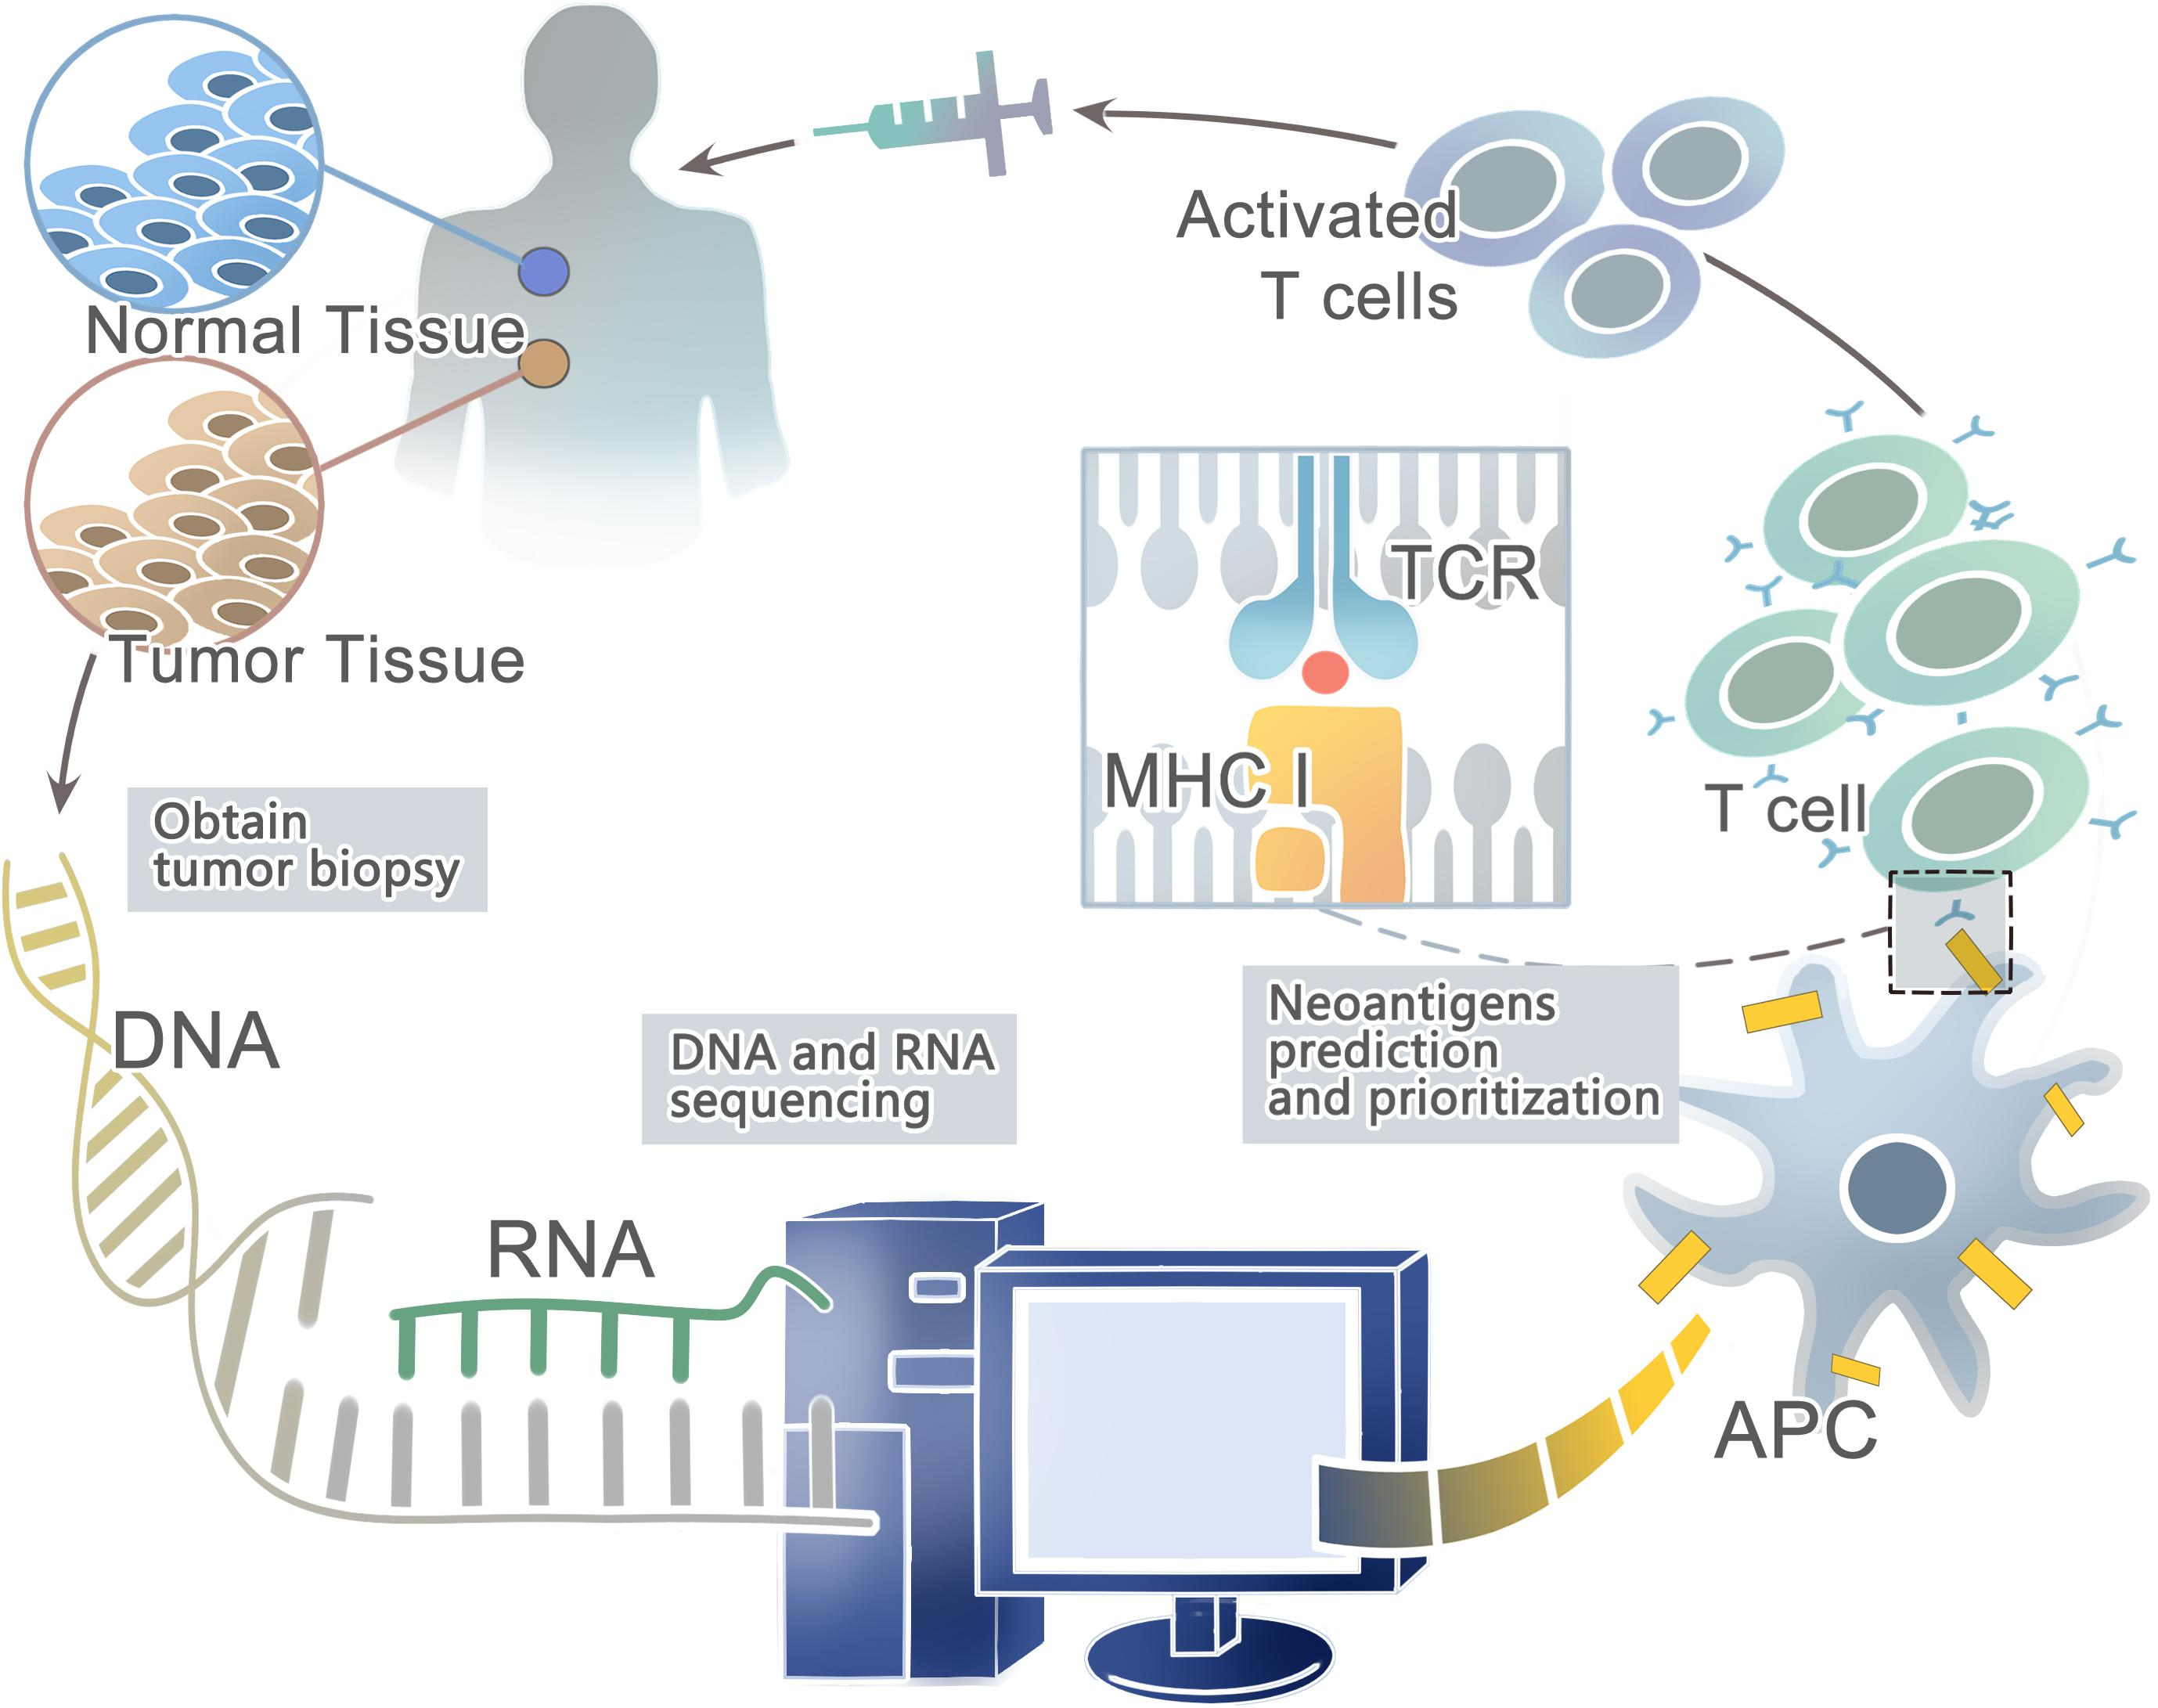
\includegraphics[width=0.45\textwidth]{../img/pipeline/vaccine_pipeline}}		
	\subfigure[Pipeline]{\label{fig:vaccines_b}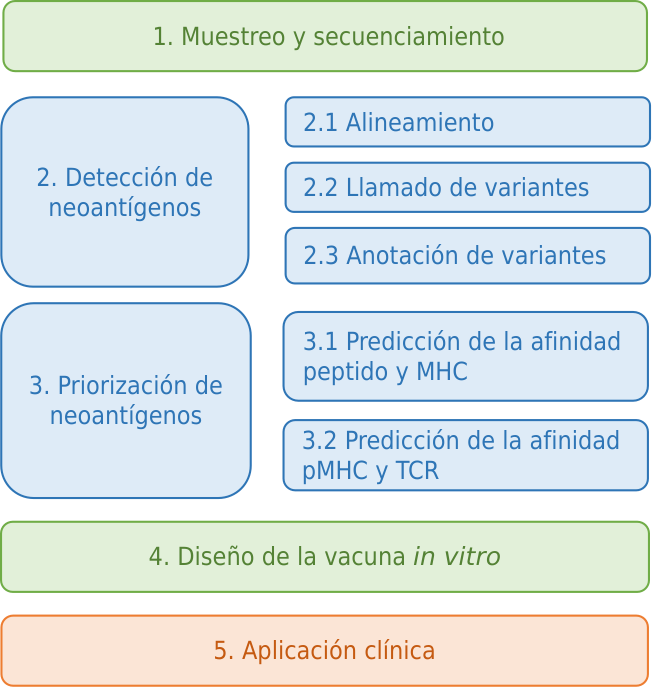
\includegraphics[width=0.45\textwidth]{img/pipeline/pipeline_spanish}}
	
	\caption[\textit{Pipeline} para el desarrollo de vacunas basadas en neoantígenos]{Marco de desarrollo para la creación de vacunas personalizadas contra el cáncer basadas en neoantígenos. (a) proporciona una visión general de cada etapa \citep{han2020progress}. (b) una visión general de cada fase con un énfasis en el desarrollo \textit{in-silico}.}
	\label{fig:vaccines}
\end{figure}

\section{Problema}
\label{sec:problema}

Los neoantígenos son péptidos mutados específicos de tumores y son considerados los principales causantes de una respuesta inmune \citep{borden2022cancer, chen2021challenges, gopanenko2020main}. Es así que surgen varios esfuerzos e investigación en la Inmunoterapia del cáncer, concentradas en el estudio y detección de neoantígenos. Es así, que el desarrollo de vacunas personalizadas basadas en neoantígenos es considerado uno de los métodos con mayor probabilidad de éxito \citep{borden2022cancer}. Incluso varias compañías como BioNTech, Genocea Biosciences, Neon Therapeutics y Gritstone Oncology realizan investigación y ofrecen el servicio de generar vacunas personalizadas a pacientes de cáncer.

Además, el MHC representa un factor clave, en la detección de neoantígenos, al ser el encargado de unirse al neoantígeno y presentarlo a la superficie de la célula. Debido a esto, este trabajo en enfoca en el desarrollo de un método para la predicción del enlace entre neoantígenos y MHC (\textit{pMHC binding}), esto corresponde a la Fase 3.1 de la Figura \ref{fig:vaccines}(b) dentro del \textit{pipeline} de detección de neoantígenos.  Existen dos tipos: el MHC clase I (MHC-I) y MHC clase II (MHC-II), ambos presentan péptidos en la superficie celular a las células T CD8+ y CD4+, respectivamente \citep{janeway1997immunobiology, abualrous2021major}. En detalle, el ciclo de vida de los neoantígenos que se unen a MHC-I se puede resumir de la siguiente manera. Primero, una proteína cancerígena se degrada en péptidos en el citoplasma. Luego, los péptidos se unen al MHC (\textit{pMHC binding}). Después, este compuesto sigue un camino hasta llegar a la membrana celular (\textit{pMHC presentation}). Finalmente, el pMHC es reconocido por el TCR, desencadenando el sistema inmunológico \citep{janeway1997immunobiology, wieczorek2017major, gasser2021interpreting}. Por lo tanto, la unión pMHC es un paso muy importante para la inmunidad celular, y la predicción y comprensión de esta unión tienen un valioso potencial. Lamentablemente, la mayoría de las ligandos pMHC no llegan a la membrana celular \citep{de2020neoantigen}. 

Adicionalmente, las proteínas MHC están codificadas por genes altamente polimórficos, llamados \textit{Antígenos Leucocitarios Humanos} (HLA); la considerable naturaleza polimórfica de los genes MHC proporciona una variación sustancial en la unión con los neoantígenos, lo que influye en el conjunto de neoantígenos presentados a las células T \citep{abualrous2021major}. En consecuencia, los métodos propuestos se categorizan como \textit{pan-specific} y \textit{allele-specific}. Los métodos \textit{allele-specific} \citep{rammensee1999syfpeithi, reche2002prediction, kim2009derivation, nielsen2016netmhcpan, vang2017hla, shao2020high, bravi2021rbm} entrenan un modelo para cada \textit{allele} del MHC; mientras que los métodos \textit{pan-specific} \citep{hu2019acme, liu2019deepseqpan, wu2019deephlapan, phloyphisut2019mhcseqnet, o2018mhcflurry, o2020mhcflurry, reynisson2020netmhcpan, venkatesh2020mhcattnnet, ye2021mathla, mei2021anthem, chu2022transformer, zhang2022hlab, mei2021anthem, hu2019acme, gfeller2023improved} entrenan un modelo global que toma péptidos (neoantígenos) y MHC como entradas. Además, la naturaleza polimórfica del MHC eleva bastante la complejidad de este problema, se cree que existen las 10000 diferentes MHC \textit{alleles} \citep{abelin2017mass}, esto complica mucho la detección de neo antígenos. Por lo tanto, los métodos \textit{pan-specific} surgen con una alta posibilidad de futuras aplicaciones.

Lamentablemente, a pesar de varios esfuerzos en el desarrollo  de métodos para la detección de neoantígenos, menos del 5\% de neoantígenos detectados activan el sistema inmune \citep{de2020neoantigen, mill2022neoms, bulik2019deep, bassani2015mass, yadav2014predicting}. Según los autores de los métodos,  las razones son: 

\begin{enumerate}
	\item La no inclusión en conjunto de varias fuentes de información como DNA-seq, RNA-seq, y datos de \textit{Mass Spectrometry} (MS) \citep{kim2018neopepsee}. Por ejemplo, la mayoría de  propuestas no utiliza datos de MS; en la actualidad, existe una creciente información de estos datos y se están aplicado a varios campos de la Bioinformática.
	\item  Uso herramientas de bajo desempeño para la predicción del enlace péptido-MHC (pMHC) (etapa 3.1  de la Figura \ref{fig:vaccines_b}). La mayoría de aplicaciones, se basa en el uso de MHCFlurry \citep{o2020mhcflurry} y NetMHCpan4.1 \citep{reynisson2020netmhcpan}. Sin embargo, actualmente, se cuenta con herramientas de mejor desempeño basado en \textit{Transformers} \citep{arceda2023neoantigen}. Esta tesis, se enfoca en resolver este problema.
	\item Para la etapa 3.2 de la Figura \ref{fig:vaccines_b}, los autores no consideran  la predicción del enlace pMHC al TCR (pMHC-TCR), varios autores consideran incluir esta tarea en trabajos futuros  \citep{rubinsteyn2018computational}.
	\item Finalmente, no utilizar información de eventos de \textit{alternative splicing}, variaciones estructurales en el ADN y las mutaciones de fusión de genes, está información esta fuertemente relacionada con varios tipos de cáncer \citep{wood2020neoepiscope}.
\end{enumerate}

En conclusión, la detección de neoantígenos es un desafío que consta de múltiples etapas, y las herramientas actuales en el estado del arte presentan un rendimiento insuficiente. Uno de los factores clave detrás de este bajo rendimiento está relacionado con la predicción del enlace pMHC. Por esta razón, esta tesis se centra en abordar este problema mediante la propuesta de un método basado en \textit{Transformers} para la predicción del enlace/unión pMHC.

%Finalmente, la detección de neoantígenos es un problema compuesto por varias etapas, y las herramientas actuales del estado del arte tiene bajo desempeño. Además, una de las principales razones del bajo desempeño esta relacionado a la predicción del enlace pMHC. Debido a eso, esta tesis, se enfoca en dar solución a este problema, proponiendo un método basado en Transformers para la predicción del enlace pMHC.

%Según lo mencionado anteriormente, la detección de neo antígenos es un factor clave en el desarrollo de vacunas personalizadas. En este proceso el compuesto \textit{Major Histocompatibility Complex} (MHC), juega un papel muy importante, es el encargado de presentar los péptidos a la células T \citep{hashemi2022improved}. Para el caso de células humanas el gen MHC es conocido como Human Leukocyte Antigens (HLA) y es polimórfico, se cree que existen las 10000 diferentes \textit{HLA-I alleles} \citep{abelin2017mass}, esto complica mucho más la detección de neo antígenos. 

%El ciclo de vida de un neo antígeno para células con núcleo podría resumirse como: primero una proteína es degradada en péptidos en el citoplasma de las células, luego los péptidos se enlazan a la molecula MHC (\textit{pMHC binding}), luego este compuesto sigue un trayecto hasta llegar a la membrana de la célula (\textit{pMHC presentation}), finalmente el compuesto pMHC es reconocido por  el T-cell Receptor (TCR) de las células T y así si activaría el sistema inmune. Además, el número de posibles péptidos enlazables a MHC  son entre 1000 a 10000, esto es el 0.1\% de los posibles péptidos  de 9 aminoacidos\footnote{La mayoría de péptidos enlazados a moléculas MHC-I tienen 9 aminoácidos, se suele utilizar el termino \textit{n-mer} para referirse a péptidos de \textit{n} aminoácidos.} \citep{abelin2017mass}. En este proceso, el objetivo es detectar los péptidos (neo antígenos) que llegan a la membrana de la célula, luego con ayuda de procedimientos de biotecnología, se entrena a las células T de un paciente para que aprenda a reconocer los neo antígenos.


%El problema de \textit{pMHC binding} está casi solucionado con una precisión de 0.98 por parte de la herramienta NetMHCPan 4.1 \citep{reynisson2020netmhcpan}. Sin embargo, no es bueno limitar la detección de neo antígenos solo al problema de \textit{pMHC binding}, porque la mayoría de estos compuestos no llegan a la membrana \citep{mill2022neoms}, a este problema se le conoce como \textit{pMHC presentation}. Por ejemplo, se sabe que menos del 5\% de péptidos detectados llegan a la membrana \citep{de2020neoantigen, mill2022neoms, bulik2019deep, bassani2015mass, yadav2014predicting}. Además, existen herramientas como NeyMHC, NetMHCpan y MHCFlurry que tienen un buen desemepeño en \textit{pMHC binding}, pero con resultados pobres en  \textit{pMHC presentation} \citep{bulik2019deep}. 



\subsection{Formulación del Problema}

El presente estudio se centra en el problema de predicción del enlace pMHC-I (\textit{pMHC binding prediction}). Esto representa un problema de clasificación binaria que toma como entrada la secuencia de aminoácidos de un péptido y el MHC. Un péptido podría representarse como: $p = \{A, ..., Q\}$ y una representación similar para el MHC sería: $q = \{A, N, ..., G\}$. Finalmente, necesitamos conocer la probabilidad de afinidad entre $p$ y $q$. Si esta probabilidad es lo suficientemente alta, es posible que el péptido se enlace al MHC y por lo tanto, el péptido $p$ en cuestión, sería un excelente candidato a neoantígeno.


%Menos del 5\% de péptidos detectados en \textit{pMHC binding}, llegan a la membrana de la células, para que luego sean reconocidos por las células T.  El proceso por el cúal un péptido enlazado a MHC llegue a la membrana es conocido como  \textit{pMHC presentation}, pero en este problema las propuestas recientes solo llegan a un 0.61 de precisión y 0.4 de \textit{recall}. Además, propuestas recientes solo llegan aun 0.6 de \textit{presicion} y 0.4 de \textit{recall} \citep{mill2022neoms}. En este contexto, la tesis se enfoca en el problema de \textit{pMHC presentation}, considerándolo como un problema de clasificación binaria, y tomando como entrada la secuencia de aminoácidos del péptido y la secuencia de aminoácidos de la proteína MHC. 



%% ------------------------------------------------------------------- %%
\section{Objetivos}
\label{sec:objetivos}

\subsection{Objetivo General}

%Detección \textit{in Silico} de Neoantígenos Utilizando \textit{Transformers} y \textit{Transfer Learning} en el Marco de Desarrollo de Vacunas Personalizadas para Tratar el Cáncer

Implementar un método \textit{in silico} basado en \textit{Transformers} y \textit{Transfer Learning} para la detección de neoantígenos, enfocados en la predicción de la unión pMHC. 

\subsection{Objetivos Específicos}

\begin{enumerate}[(a)]
	%\item Analizar herramientas del estado del arte como: NetMHCpan4.1, MHCFlurry2.0, Anthem, ACME y MixMHCpred2.2, utilizadas para la predicción del enlace pMHC en el contexto de detección de neonatígenos.
	\item Analizar los métodos que utilizan \textit{Transformers} para la predicción del enlace pMHC en el contexto de detección de neoantígenos.
	\item Analizar los modelos basados en \textit{Transformers} TAPE, ProtBert-BFD, y EMS2 pre-entrenados para diversas tareas en Proteómica y de los cuáles se puede aplicar \textit{Transfer Learning}. 	
	\item Implementar \textit{fine-tuning} a los modelos TAPE, ProtBert-BFD, y EMS2 para la tarea de predicción del enlace pMHC, aplicando \textit{Gradient Accumulation Steps} (GAS) y una metodología de congelamiento de capas.
	\item Comparar los modelos de mejor desempeño con las herramientas del estado del arte como: NetMHCpan4.1, MHCFlurry2.0, Anthem, ACME y MixMHCpred2.2.
%\item Realizar una revisión sistemática de la literatura e implementar los métodos con mejor desempeño en la detección de neo antígenos.
%\item Proponer e implementar un método basado en \textit{deep learning} para la detección de neo antígenos.		
%\item Evaluar el método propuesto en bases de datos publicas.
\end{enumerate}

%% ------------------------------------------------------------------- %%
\section{Contribuciones}
\label{sec:contribuciones}
Las principales contribuciones de este trabajo son:

\begin{enumerate}[(a)]
	\item Revisión y análisis de los métodos basados en \textit{Transformers} para la detección de neoantígenos. Se cuenta con dos publicaciones: \textit{``Deep Learning and Transformers in MHC-Peptide Binding and Presentation Towards Personalized Vaccines in Cancer Immunology: A Brief Review''} \citep{machaca2023deep} y \textit{``Transformers Meets Neoantigen Detection: A Systematic Literature Review''}.
	\item \textit{Fine-tuning} a seis modelos de \textit{Transformers} para la predicción del enlace pMHC; además, se ha evaluado el uso de GAS y una metodología de congelamiento de capas. Se cuenta con dos publicaciones: \textit{``Neoantigen Detection Using Transformers and Transfer Learning in the Cancer Immunology Context''} \citep{arceda2023neoantigen} y \textit{``Fine-tuning Transformers for Peptide-MHC Class I Binding Prediction''}.
	\item Comparación de los métodos propuestos con herramientas del estado del arte como: NetMHCpan4.1, MHCFlurry2.0, Anthem, ACME y MixMHCpred2.2. Los métodos propuestos tienen los mejores resultados en \textit{accuracy}, \textit{Area Under the Curve} (AUC), \textit{recall}, \textit{f1-score} y \textit{Matthews Correlation Coefficient}  (MCC).
\end{enumerate}

\clearpage
%% ------------------------------------------------------------------- %%
\section{Organización del Trabajo}
\label{sec:organizaciondeltrabajo}

El restante de este trabajo está organizado de la siguiente manera:

\begin{itemize}
	\item En el Capítulo \ref{cap:marcoteorico} se presentan los conceptos básicos sobre Bioinformática e inmunoterapia del Cáncer, también son abordados temas sobre \textit{Deep Learning} y redes neuronales \textit{Transformers}.
	
	\item Luego, en el Capítulo \ref{cap:estadodelarte} se describen los trabajos relacionados a la presente tesis. Debido a la gran cantidad de publicaciones, solo se ha considerado trabajos desde el 2018 y que hacen uso de \textit{Transformers} o redes neuronales con mecanismos de atención.
	
	\item El Capitulo \ref{cap:propuesta}, presenta la propuesta de la tesis. Esta se basa en un método para desarrollar \textit{fine-tuning} a \textit{Transformers} pre-entrenados para diversas tareas de Proteómica. 
	
	\item Luego, en el Capítulo  \ref{cap:resultados}, se presentan los resultados de la investigación. Además, se presenta una comparación con los métodos del estado del arte.
	
	\item Finalmente, en el Capítulo~\ref{cap:conclusiones} son expuestos las conclusiones del presente trabajo así como también las direcciones para continuar con el mismo en la sección de trabajos futuros.
	
	
	
\end{itemize}





%Em anexos está uma exemplificação da especificação da arquitetura, 
%neste caso é descrita a especificação da arquitetura 
%DAS-3 (Apêndice \ref{ape:especificacoes}).


%%%%%
